\subsection{Database}
The data layer must contain the DB and also a DBMS component necessary to manage all possible operation, such as insertion, deletion, update, that can be done on data inside the storage unit. The chosen DBMS must guarantee the correct working of transaction according to the ACID properties.\\A RDBMS is the best choice for this app because it adheres to the ACID properties; guarantees high performances by using indexis to sort data and by supporting both desktop and web apps and also guarantees data security providing a layer of protection for sensitive data. Using a RDBMS it is also possible to build  the DB structure and clearly define the relations between data.\\ As said in the previous section, the chosen architecture is composed by closed layers and for this reason  the data layer, the one which contains the stored data, can only be accessed by the Application's one, via a dedicated interface. Bacause of this it is necessary to provide a persistence unit which can handle all possible behaviors. Credentials and sensible data as personal informations must be encripted to avoid any possible privacy violation.\\
The Entity Relational diagram in figure describe a first relational model of the Database. The rectangual shapes represent the entities; the circles all possible attributes related to an entity in particular all cirles filled in black are the entities key and the relationships are represented by diamonds.

\begin{figure}[h!]
	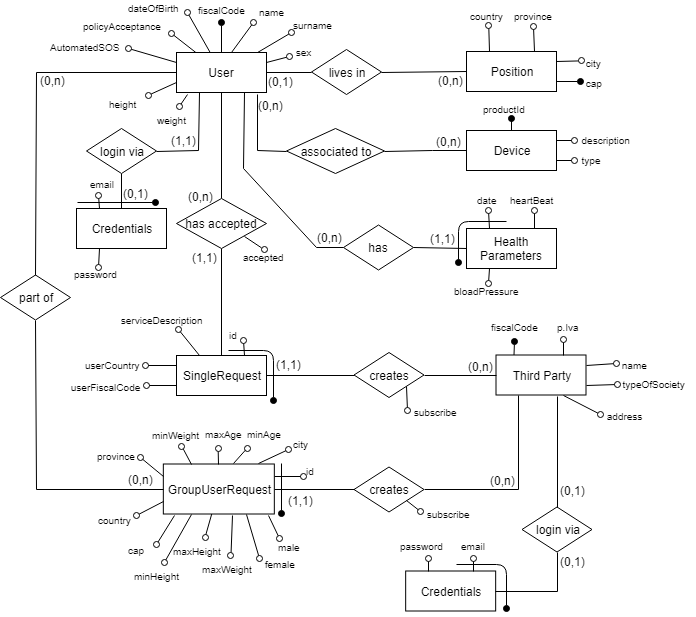
\includegraphics[width=1.20\textwidth]{./pictures/ER_diagram.png}\par
	\caption{Entity Relationship diagram}
\end{figure}
\FloatBarrier